\documentclass[tikz]{standalone}

\begin{document}
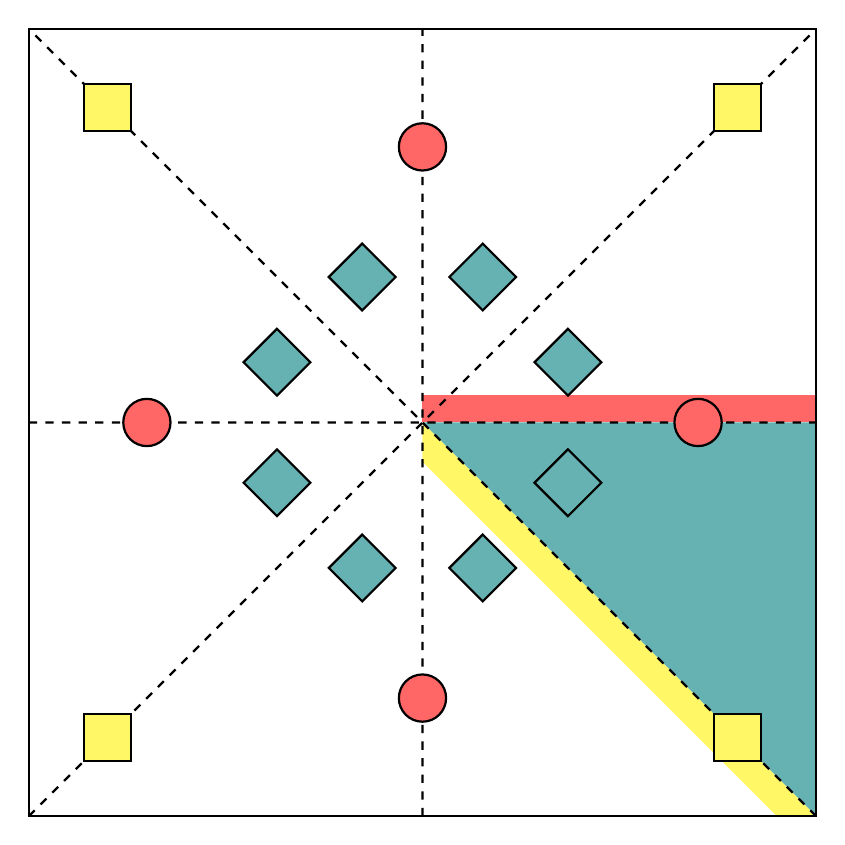
\begin{tikzpicture}[thick]
  \def\r{5}
  \fill[teal!60] (\r,-\r) -- (0,0) -- (\r,0) -- cycle;
  \fill[yellow!60] (\r,-\r) -- (0,0) -- (0,-0.\r) -- (4.\r,-\r) -- cycle;
  \fill[red!60] (0,0) rectangle (\r,0.3\r);
  \draw (-\r,-\r) rectangle (\r,\r);
  \draw[dashed] (-\r,-\r) -- (\r,\r) (\r,-\r) -- (-\r,\r) (-\r,0) -- (\r,0) (0,-\r) -- (0,\r);

  \foreach \a in {-0.8*\r,0.8*\r}
  \foreach \b in {-0.8*\r,0.8*\r}
  \draw[fill=yellow!60] (\a,\b) +(-0.3,-0.3) rectangle +(0.3,0.3);

  \foreach \a in {-0.7*\r,0.7*\r} {
      \draw[fill=red!60] (\a,0) circle (0.3);
      \draw[fill=red!60] (0,\a) circle (0.3);
    }

  \foreach \i in {1,...,8}
  \draw[rotate=45,fill=teal!60] (\i*360/8+22.5:2cm) +(-0.3,-0.3) rectangle +(0.3,0.3);
\end{tikzpicture}
\end{document}
